\input{../preamble.tex}
% \bibliographystyle{plain} % Style BST file (bmc-mathphys, vancouver, spbasic).
% \bibliographystyle{unsrt} % Style BST file (bmc-mathphys, vancouver, spbasic).
\bibliography{pubs.bib}      % Bibliography 

\title{Professional Drone, Hybrid Power Pack  - Timebox 9}
\author{Team 2}

\begin{document}

\lstset{language=Matlab,%
  % basicstyle=\color{red},
    inputencoding=latin1,
    breaklines=true,%
    morekeywords={matlab2tikz},
    keywordstyle=\color{blue},%
    morekeywords=[2]{1}, keywordstyle=[2]{\color{black}},
    identifierstyle=\color{black},%
    stringstyle=\color{mylilas},
    commentstyle=\color{mygreen},%
    showstringspaces=false,%without this there will be a symbol in the places where there is a space
    numbers=left,%
    numberstyle={\tiny \color{black}},% size of the numbers
    numbersep=9pt, % this defines how far the numbers are from the text
    emph=[1]{for,end,break},emphstyle=[1]\color{red}, %some words to emphasise
    %emph=[2]{word1,word2}, emphstyle=[2]{style},    
}


\lstset{language=C,%
  % basicstyle=\color{red},
  inputencoding=latin1,
  breaklines=true,%
  morekeywords={matlab2tikz},
  keywordstyle=\color{blue},%
  morekeywords=[2]{1}, keywordstyle=[2]{\color{black}},
  identifierstyle=\color{black},%
  stringstyle=\color{mylilas},
  commentstyle=\color{mygreen},%
  showstringspaces=false,%without this there will be a symbol in the places where there is a space
  % numbers=left,%
  % numberstyle={\tiny \color{black}},% size of the numbers
  % numbersep=9pt, % this defines how far the numbers are from the text
  emph=[1]{for,end,break},emphstyle=[1]\color{red}, %some words to emphasise
  % emph=[2]{word1,word2}, emphstyle=[2]{style},
}


% \lstdefinestyle{customc}{
%   belowcaptionskip=1\baselineskip,
%   breaklines=true,
%   frame=L,
%   xleftmargin=\parindent,
%   language=C,
%   showstringspaces=false,
%   basicstyle=\footnotesize\ttfamily,
%   keywordstyle=\bfseries\color{green!40!black},
%   commentstyle=\itshape\color{purple!40!black},
%   identifierstyle=\color{blue},
%   stringstyle=\color{orange},
% }

% \lstdefinestyle{customasm}{
%   belowcaptionskip=1\baselineskip,
%   frame=L,
%   xleftmargin=\parindent,
%   language=[x86masm]Assembler,
%   basicstyle=\footnotesize\ttfamily,
%   commentstyle=\itshape\color{purple!40!black},
% }

% \lstset{escapechar=@,style=customc}

\newcounter{udrboks}[section]\setcounter{udrboks}{0}
\renewcommand{\theudrboks}{\arabic{section}.\arabic{udrboks}}
\renewcommand{\theudrboks}{\arabic{udrboks}}
\newenvironment{udrboks}[2][]{%
  \refstepcounter{udrboks}%
  \ifstrempty{#1}%
  {\mdfsetup{%
      frametitle={%
        \tikz[baseline=(current bounding box.east),outer sep=0pt]
        \node[anchor=east,rectangle,fill=blue!20]
        {\strut Udregninger~\theudrboks};}}
  }%
  {\mdfsetup{%
      frametitle={%
        \tikz[baseline=(current bounding box.east),outer sep=0pt]
        \node[anchor=east,rectangle,fill=blue!20]
        {\strut Udregninger ~\theudrboks:~#1};}}%
  }%
  \mdfsetup{innertopmargin=10pt,linecolor=blue!20,%
    linewidth=2pt,topline=true,%
    frametitleaboveskip=\dimexpr-\ht\strutbox\relax
  }
  \begin{mdframed}[]\relax%
    \label{#2}}{\end{mdframed}}


\newcounter{formelboks}[section]\setcounter{formelboks}{0}
\renewcommand{\theformelboks}{\arabic{section}.\arabic{formelboks}}
\renewcommand{\theformelboks}{\arabic{formelboks}}
\newenvironment{formelboks}[2][]{%
  \refstepcounter{formelboks}%
  \ifstrempty{#1}%
  {\mdfsetup{%
      frametitle={%
        \tikz[baseline=(current bounding box.east),outer sep=0pt]
        \node[anchor=east,rectangle,fill=blue!20]
        {\strut Formler~\theformelboks};}}
  }%
  {\mdfsetup{%
      frametitle={%
        \tikz[baseline=(current bounding box.east),outer sep=0pt]
        \node[anchor=east,rectangle,fill=blue!20]
        {\strut Formler ~\theformelboks:~#1};}}%
  }%
  \mdfsetup{innertopmargin=10pt,linecolor=blue!20,%
    linewidth=2pt,topline=true,%
    frametitleaboveskip=\dimexpr-\ht\strutbox\relax
  }
  \begin{mdframed}[]\relax%
    \label{#2}}{\end{mdframed}}

\newcounter{konstboks}[section]\setcounter{konstboks}{0}
\renewcommand{\thekonstboks}{\arabic{section}.\arabic{konstboks}}
\newenvironment{konstboks}[2][]{%
  \refstepcounter{konstboks}%
  \ifstrempty{#1}%
  {\mdfsetup{%
      frametitle={%
        \tikz[baseline=(current bounding box.east),outer sep=0pt]
        \node[anchor=east,rectangle,fill=green!20]
        {\strut Konstanter~\thekonstboks};}}
  }%
  {\mdfsetup{%
      frametitle={%
        \tikz[baseline=(current bounding box.east),outer sep=0pt]
        \node[anchor=east,rectangle,fill=green!20]
        {\strut Konstanter~\thekonstboks:~#1};}}%
  }%
  \mdfsetup{innertopmargin=10pt,linecolor=green!20,%
    linewidth=2pt,topline=true,%
    frametitleaboveskip=\dimexpr-\ht\strutbox\relax
  }
  \begin{mdframed}[]\relax%
    \label{#2}}{\end{mdframed}}
\pgfplotstableread[row sep=\\,col sep=&]{
  ide & stemmer  \\
  Paraply & 9  \\
  Fjernbetjening & 7  \\
  iAdapt & 2 \\
}\mydata
% \setcounter{secnumdepth}{1}
\maketitle
\thispagestyle{empty}

\textbf{Deltagere:}
\begin{figure}[h]
  \centering
  % BEGIN RECEIVE ORGTBL delt
  \begin{tabular}{|p{5cm}p{10cm}|}
    \hline
    &\\
    Stud. nr: 201602094 & Navn: Søren Holm Korsgaard \\
    \hline
    &\\
    Stud.nr.: 201607563 & Navn: Jacob Gustafsson \\
    \hline
    &\\
    % Stud.nr.: 201704859 & Navn: Jonas Buus \\
    % \hline
    % &\\
    Stud.nr.: 20084327 & Navn: Simon Rasmussen \\
    \hline
    &\\
    Stud.nr.: 201704483 & Navn: Thomas Dueholm Jensen \\
    \hline
  \end{tabular}
  % END RECEIVE ORGTBL delt

\end{figure}
\vspace{-5mm}
% \clearpage
\setcounter{tocdepth}{2}
\tableofcontents
\thispagestyle{empty}
\newpage
% \pagenumbering{arabic}
\setcounter{page}{1}

% \section{Introduktion}
% \label{sec:introduktion}

\section{Strategy and planning (Jacob)}
\label{sec:strat-plann-jacob}

\subsection{Strategy}
\label{sec:strategy}


I timebox 9 har vi planlagt at færdiggøre de resterende hardwaresystemer, så disse er testet og klar til implementering. Dette indebærer også, at vi skal have lagt os fast på et interface mellem ensretteren og batteriet. For PID-reguleringens vedkommende, er det planen at der skal simuleres i SimuLink.

\subsection{Planning}
\label{sec:planning}


\subsubsection{PID-regulering}
\label{sec:pid-regulering}

I denne timebox gennemgås tuning af PID-koefficienterne og næste timebox vil indeholde implementering af PID-reguleringen.

\subsubsection{Ensretter}
\label{sec:ensretter}


Ensretteren har gennemgået test i denne timebox. I næste timebox er vi klar til at analysere interface og tilslutte ensretteren til det endelige system. 

\subsubsection{Spændingsregulator }
\label{sec:spandingsregulator-}


Spændingsregulatoren er endeligt testet i denne timebox. I timebox 10 skal der for spændingsregulatoren analyseres interface og tilsluttes til det endelige system. 

\subsubsection{Fuldt system }
\label{sec:fuldt-system-}

I timebox 10 tester vi det endelige system på hardwarebasis. Tester at alle interface fungerer og at de enkelte subsystemer fungerer med hinanden. 
\clearpage
\section{Spændingsregulator (Jacob) }
\label{sec:spand-jacob-}

I denne timebox er spændingsregulatoren blevet loddet op og testet. 

\subsection{Testen }
\label{sec:testen-}

Spændingsregulatoren blev meget enkelt testet ved at tilslutte en strømforsyning som input og tilslutte et voltmeter, for at måle udgangsspændingen. Opstillingen kan ses herunder. 
\begin{figure}[h]
  \centering
  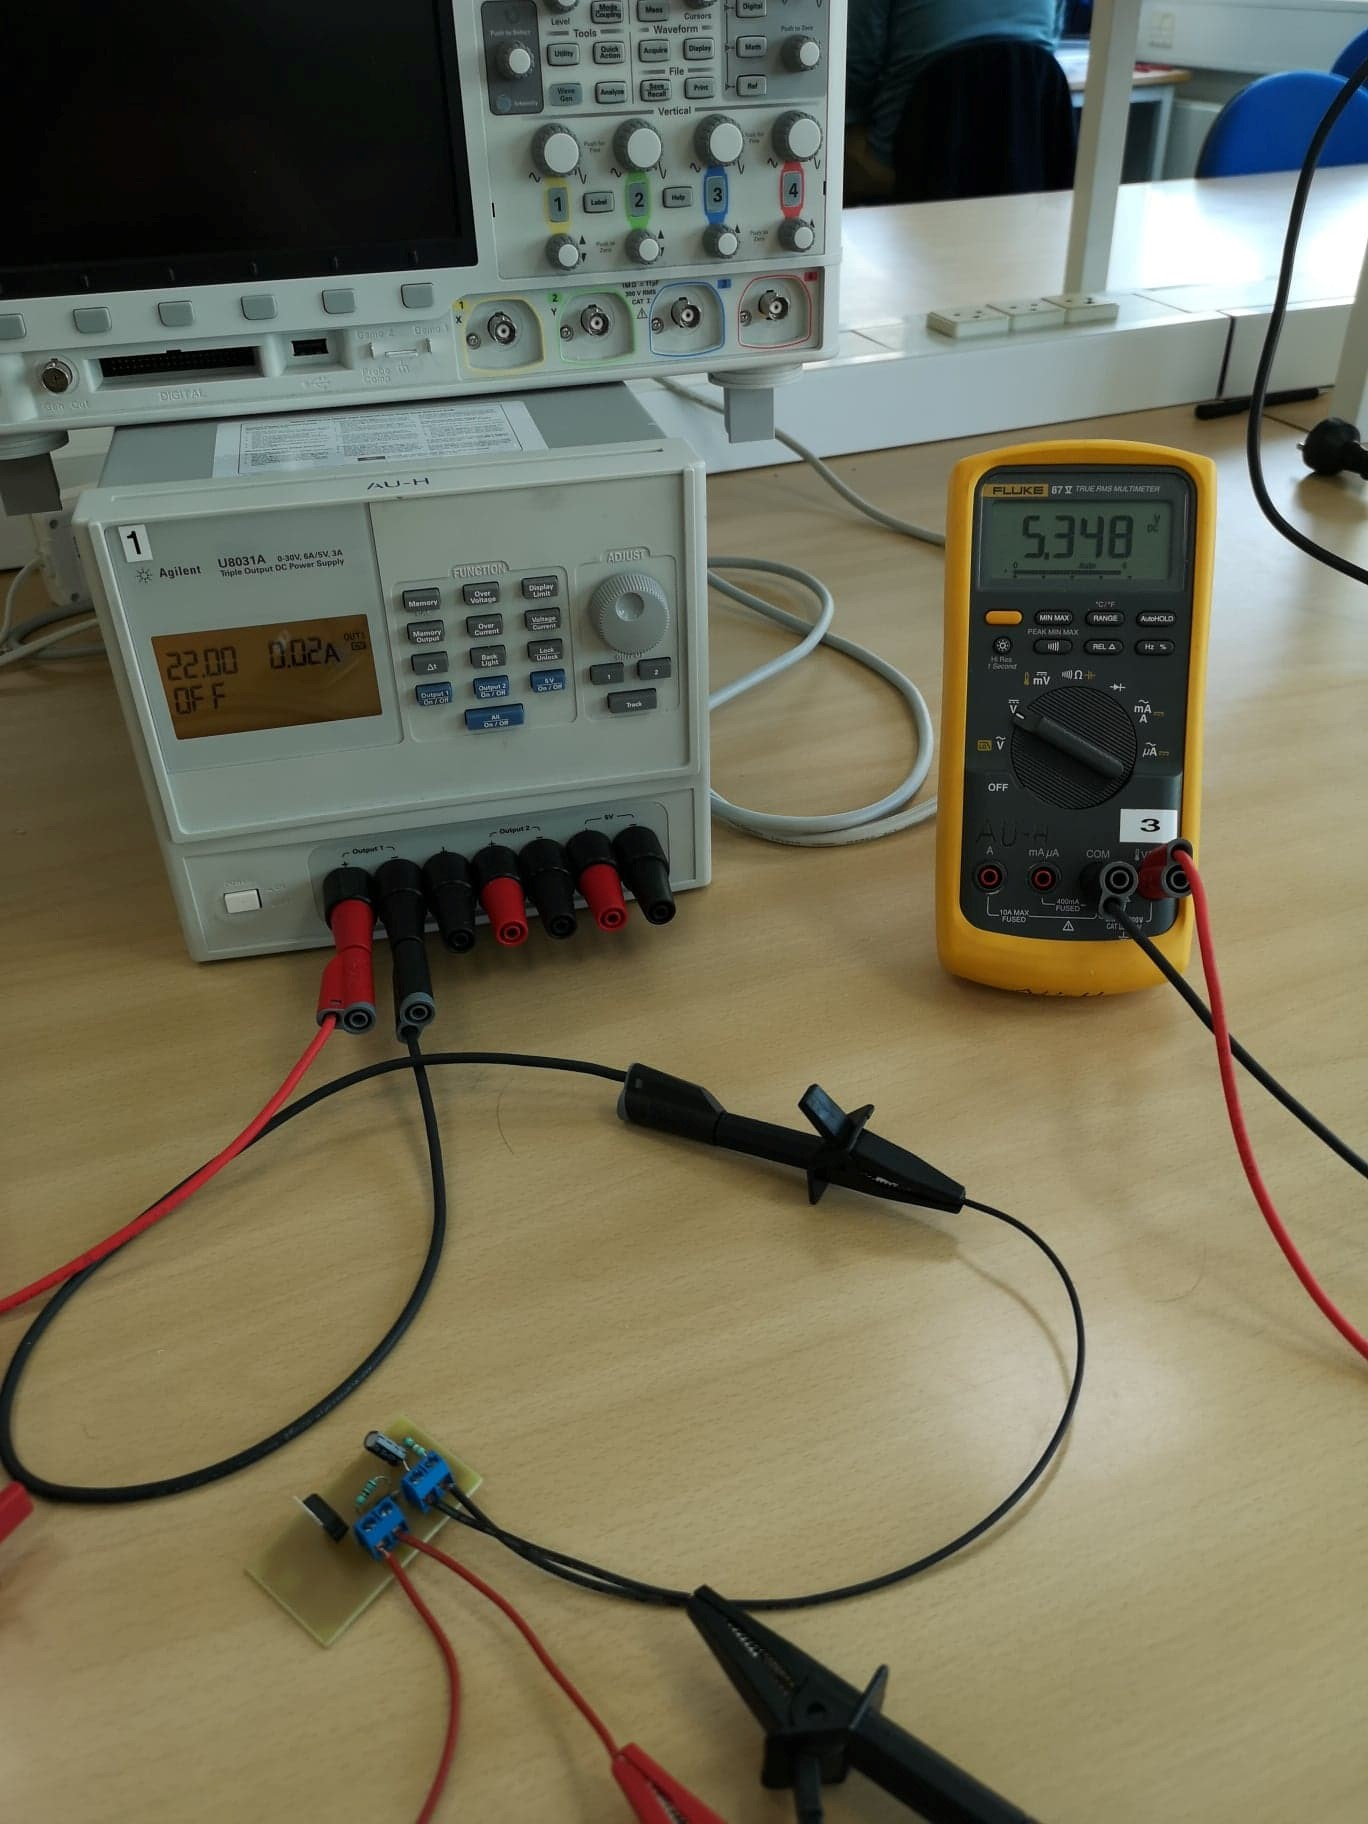
\includegraphics[width=0.6\textwidth]{jbil1.jpg}
  \caption{Testen}
  \label{fig:jbil1}
\end{figure}

\subsection{Resultater og konklusion }
\label{sec:result-og-konkl}

Som det fremgår af ovenstående billede, regulerer spændingsregulatoren fra 22 V til 5,3 V. Output spændingen er altså en smule højere end tilsigtet, men ikke mere end det kan fungere. Da setuppet blev bygget på breadboard var outputspændingen på 5,1 V. Forskellen ligger i, at der er en større intern modstand på breadboardet end på PCB-printet, hvilket der ikke er blevet taget højde for. 
\clearpage
\section{Ammendment til TB8}
\label{sec:ammendment-til-tb8}

\subsection{Intro}
\label{sec:intro}

Efter forespørgsel fra kunden, følger hermed et par tilføjelser til afsnittet om spændingsregulatoren i Timebox 8. 
Kundne har forespurgt på prisen på de specifikke komponenter, samt en beregning af udviklingen af varme fra LM317. 

\subsection{Priserne}
\label{sec:priserne}

I tidligere timebox, blev priserne på elementer der allerede var tilgængelige angivet til DKR 0,-. Herunder følger den opdaterede prisliste.

\begin{table}[h]
  \centering
% BEGIN RECEIVE ORGTBL tabel1
\begin{tabular}{ll}
\hline
Komponent & Pris i DKR \\
\hline
LM317-T (erstatter LM117-HVH) & 3,4 \\
\hline
Kondensator & 0,15 \\
\hline
Variabel modstand & 5,95 \\
\hline
Modstand & 0,65 \\
\hline
Diode & 0,36 \\
\hline
IALT & 10,51 \\
\hline
\end{tabular}
% END RECEIVE ORGTBL tabel1
  \caption{Kompenenter}
  \label{tab:komp}
\end{table}

\subsection{Varmeudvikling}
\label{sec:varmeudvikling}

Ligeledes efterspørges en beregning af varmeudviklingen fra LM317. Beregningen følger herunder. 
Da spændingsregulatoren på nuværende tidspunkt er installeret i systemet og derfor ikke er mig tilgængeligt, tages der udgangspunkt i nedenstående simulering. Simuleringen bruges til at estimere effekttabet i LM317. 

\begin{figure}[h]
  \centering
  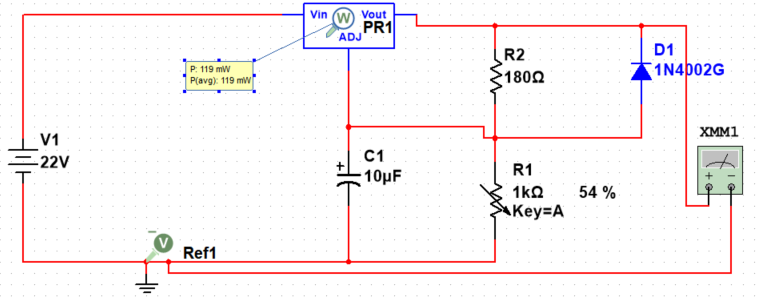
\includegraphics[width=0.6\textwidth]{jbilx.png}
  \caption{}
  \label{fig:jbilx}
\end{figure}

Som det ses af ovenstående billede, afsættes der 119 mW i komponenten.

Af datashettetet\footnote{http://www.ti.com/lit/ds/symlink/lm317.pdf} fremgår det, at $R_(\theta(JA))$ for vores pakke (TO-220) LM317KCT er 37,9 $^\circ C/W$. Vi afsætter cirka 119 mW, og dermed bliver varmeudledningen som følger: 

\begin{equation}
  \label{eq:3}
  \Delta \tau = R_{\theta (JA)}\cdot P = 37,9 \frac{^\circ C}{W}\cdot 119mW\approx 4,5101 ^\circ C
\end{equation}

Af beregningen fremgår det altså, at temperaturen stiger minimalt. 
Dette stemmer meget godt overens med, at jeg ikke kunne føle nogen forskel i temperaturen på komponenten, efter regulatoren havde kørt i 30 minutter kontinuert. 

\clearpage
\section{Aflæsning af RPM (Søren)}
\label{sec:aflasning-af-rpm}

Implementering af kode til at aflæse rpm, der skal bruges til vores PID-regulering. Vi har taget udgangspunkt i aflæse et tacho signal som kommer fra vores tændspole. Dette signal lave en høj spænding ved hver omdr, og går lav igen. 

For at afkode dette signal, bruges der input capture, der er implementeret i TPM periferenheden på kl25. Funktionen input capture, fungere ved at den tælle op til hver ’rising edge’ og gemmer denne værdi. Og når vi kender værdien og frekvensen vi tæller op med, kan vi omregne dette til RPM. 

Ved formlen: $\frac{\mathrm{60\ sek}\cdot\mathrm{frekvens}}{input\ capture\ værdien} = RPM$.

Selve koden er vist her forneden, hvor vi bruger interrupts, til at opfange overflows og når vi får et rising edge, gemmer den værdi i CNV-registeret.

\lstinputlisting[firstline=37,lastline=56]{rpm-detect.c}

Her initialiseres vores TPM1 modul. Vores frekvens der bruges til at tælle op med, bliver nedskaleret, til 375 kHz. Dvs. imellem hver overflows går der 5,75 Hz, hvilket passer med vores måle område (17 - 167 Hz) vi arbejder i. 
Ved testen, simuleret vi et tastesignal med frekvensen 10 Hz, og kunne decode det til 600 RPM -+ 20. Da der var lidt støj på signalet.

\lstinputlisting[firstline=7,lastline=36]{rpm-detect.c}

Her ses vores handler, hvori RPM bliver beregnet ud fra værdierne fra TPM1 perifer enhed. Og videre i koden kan man detektere om der er kommet ny RPM-data, ved bruge enum ’state’. Da det tager minimum en omgang på krumtappen, før den har beregnet en ny værdi.
\clearpage

\section{Funktionalitetstest af aktiv ensretter. (Thomas)}
\label{sec:funkt-af-aktiv}

For at teste funktionalitet af det færdig-loddede PCB print til den aktive ensretter, besluttede vi os for at lave en måling af $V_{in}$, fase 1, vs. $V_{out}$. Ved at sammenligne niveauet på kredsløbets udgangsspænding med niveauet på indgangen, vil det være muligt at se det samlede spændingstab gennem kredsløbet. Dette spændingstab skal være under 0.7 volt, for at kredsløbet er en forbedring i forhold til en almindelig ensretter bestående af en diodebro. 
Målingen foretages med et tilgængeligt oscilloskop fra El-lab i AU Herning, hvor data fra målingen eksporteres til en .csv fil. Med .csv filen er muligt at behandle signalerne i programmet, Matlab.

På nedenstående figur ses et diagram over kredsløbet til den aktive ensretter for at vise, hvor måleproberne er placeret under målingen.

\begin{figure}[h]
  \centering
  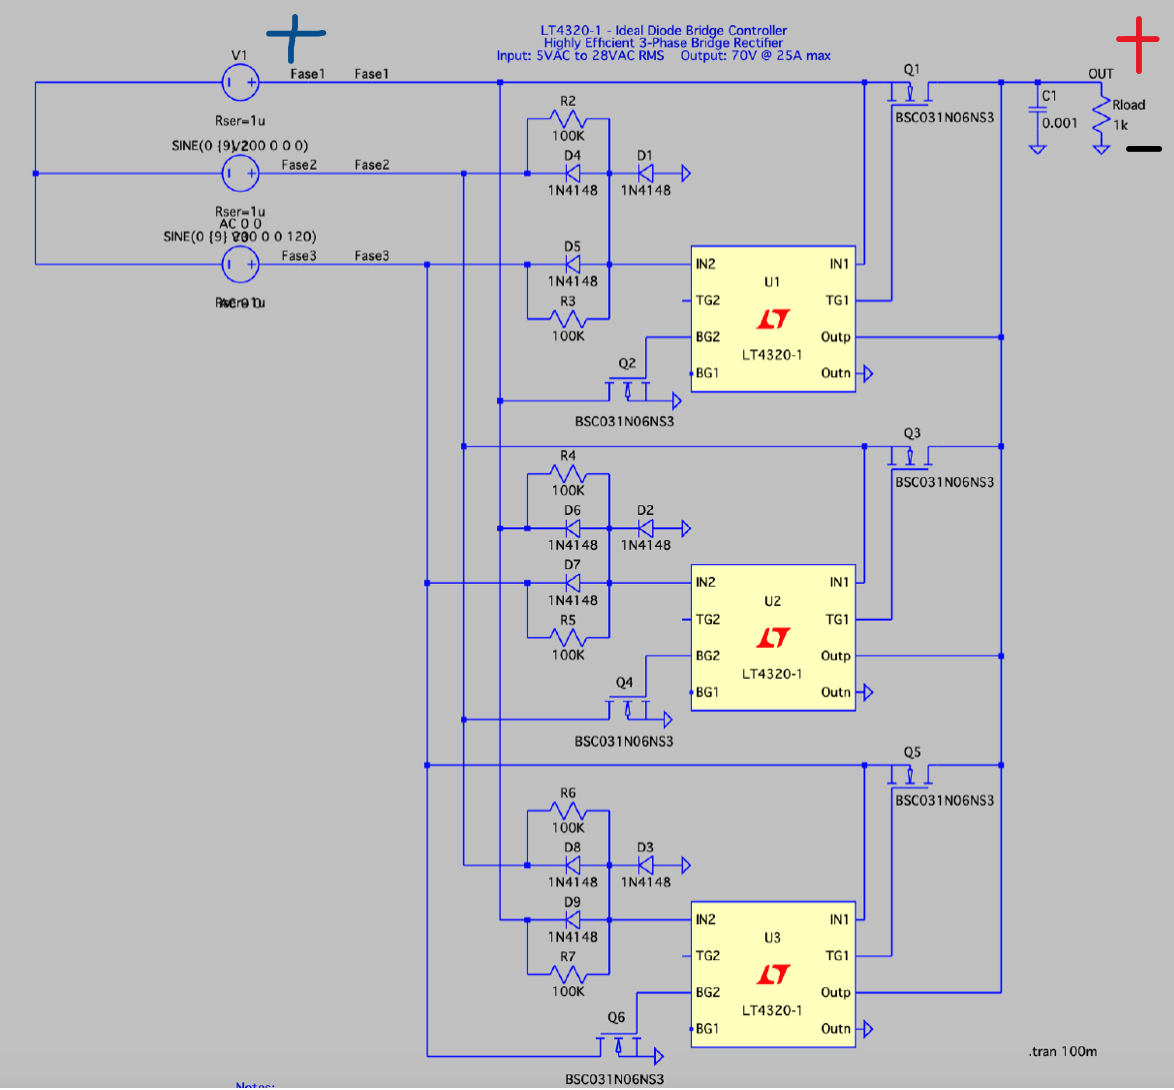
\includegraphics[width=0.6\textwidth]{tbil1.png}
  \caption{Blå: Probe 1 (Fase 1). Rød: Probe 2 ($V_{out}$)}
  \label{fig:jbil1}
\end{figure}

Teststanden fra timebox 7 benyttes til at generere en 3 faset spænding, som sendes ind i den aktive ensretter. Der er benyttet en loadmodstand på 1 k$\Omega$, ligesom der er monteret en kondensator på 1000 $\mu$F parallelt med loadmodstanden for at udglatte outputspændingen. 

Der blev foretaget 2 målingen. Én hvor generatoren producerede ca. 14.5 V (peak), og én hvor der produceres ca. 10 V (peak). Efter den fysiske måling blev data importeret i Matlab, hvor signalerne blev midlet med et medianfilter. Herefter plottes signalerne for at udfinde det segment, hvor fasen er større end outputtet.

Nedenstående figurer (\ref{fig:matcode2}-\ref{fig:tbil3}) viser Matlab scriptet, der blev benyttet til databehandlingen, samt plots af de to målinger.
\clearpage
\begin{figure}[h]
  \centering
\lstinputlisting[language=Matlab,firstline=8,lastline=30]{vin-vs-vout.m}
%   \caption{Matlab script.}
%   \label{fig:matcode}
% \end{figure}

% \begin{figure}[h]
%   \centering
\lstinputlisting[language=Matlab,firstline=29,lastline=48]{vin-vs-vout.m}  
  \caption{Matlab script.}
  \label{fig:matcode2}
\end{figure}
\clearpage
\begin{figure}[h]
  \centering
  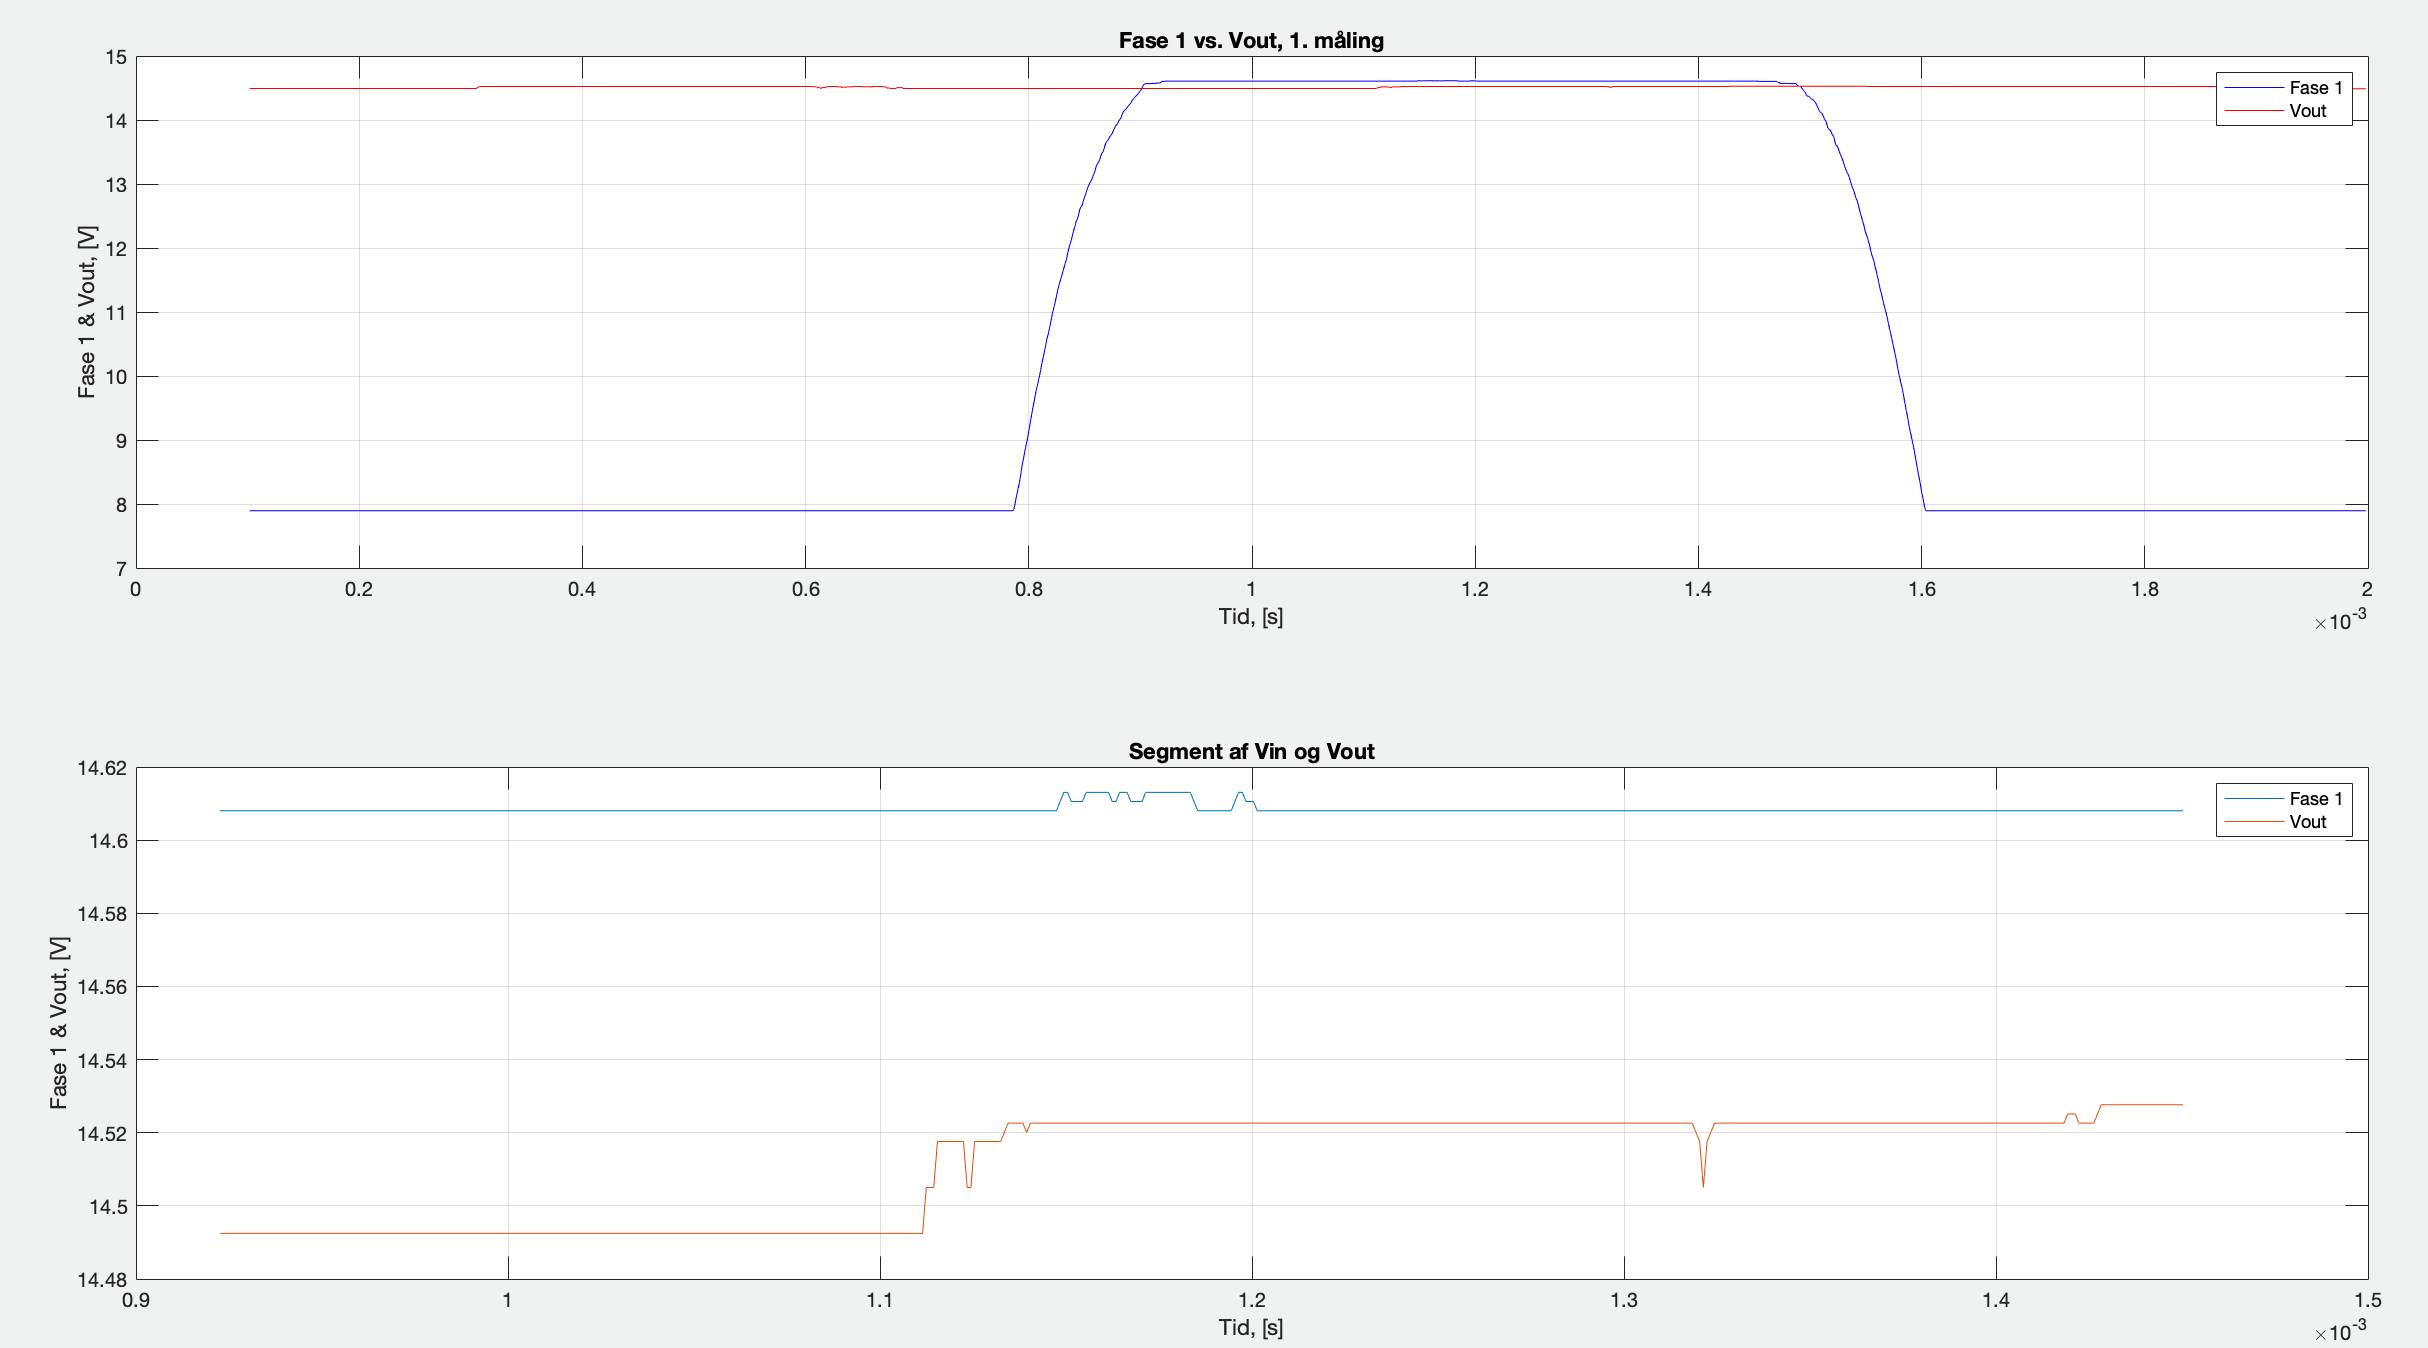
\includegraphics[width=0.6\textwidth]{tbil2.png}
  \caption{Første måling ($V_{in}$ = 14.613 [V], $V_{out}$ = 14.528 [V])}
  \label{fig:tbil2}
\end{figure}

\begin{figure}[h]
  \centering
  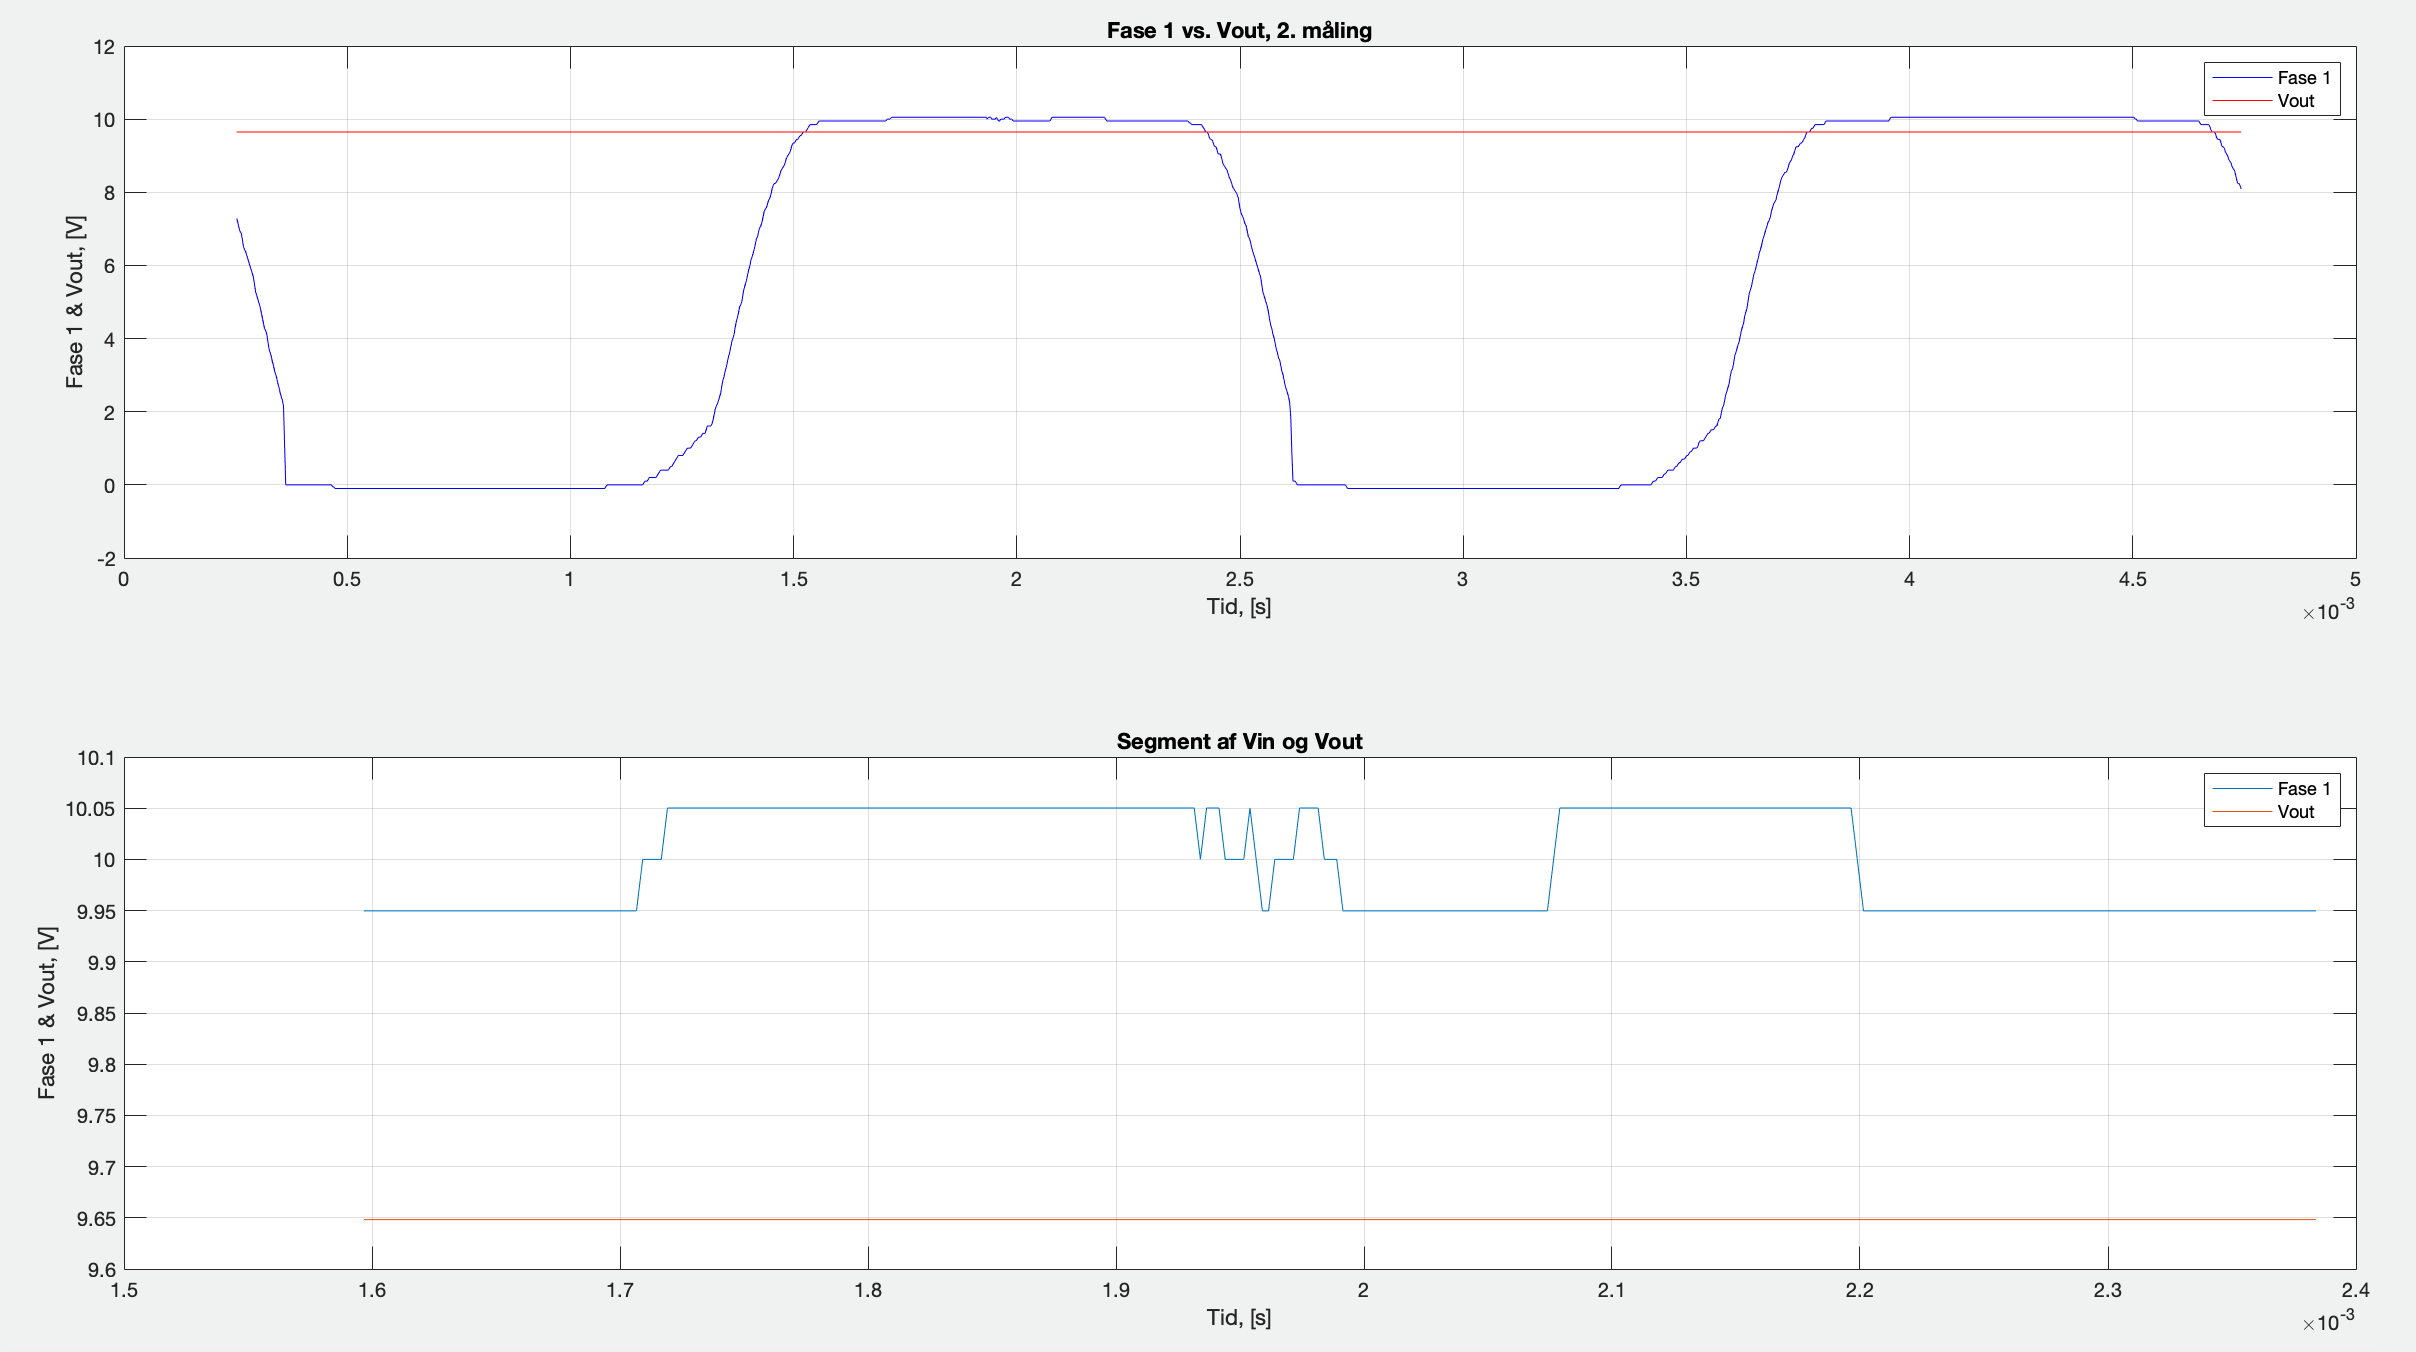
\includegraphics[width=0.6\textwidth]{tbil3.png}
  \caption{Anden måling ($V_ {in}$ = 10.050 [V], $V_{out}$ = 9.648 [V])}
  \label{fig:tbil3}
\end{figure}

Som det ses ud fra begge plots i figur 4 og 5, er der et spændingstab på udgangen af ensretteren i forhold til indgangen. Spændingstabene for målingerne er i Matlab udregnet til:

\begin{enumerate}
\item måling:	Vdelta1 = 0.0967 volt
\item måling:	Vdelta2 = 0.3497 volt
\end{enumerate}

\subsection{Større load}
\label{sec:storre-load}

For at teste om ensretter kredsløbet kan leve op til de store strømme (80 A peak), som det færdige HPP system teoretisk set kan komme til at trække, er der anskaffet en effektmodstand på ca. 12 m$\Omega$. Denne effektmodstand kan håndtere op til 25 A. Kredsløbet kan ikke testes fuldt ud med denne modstand, men det vil give en indikation af, hvordan kredsløbet reagerer ved en større belastning.
\clearpage
\begin{figure}[h]
  \centering
  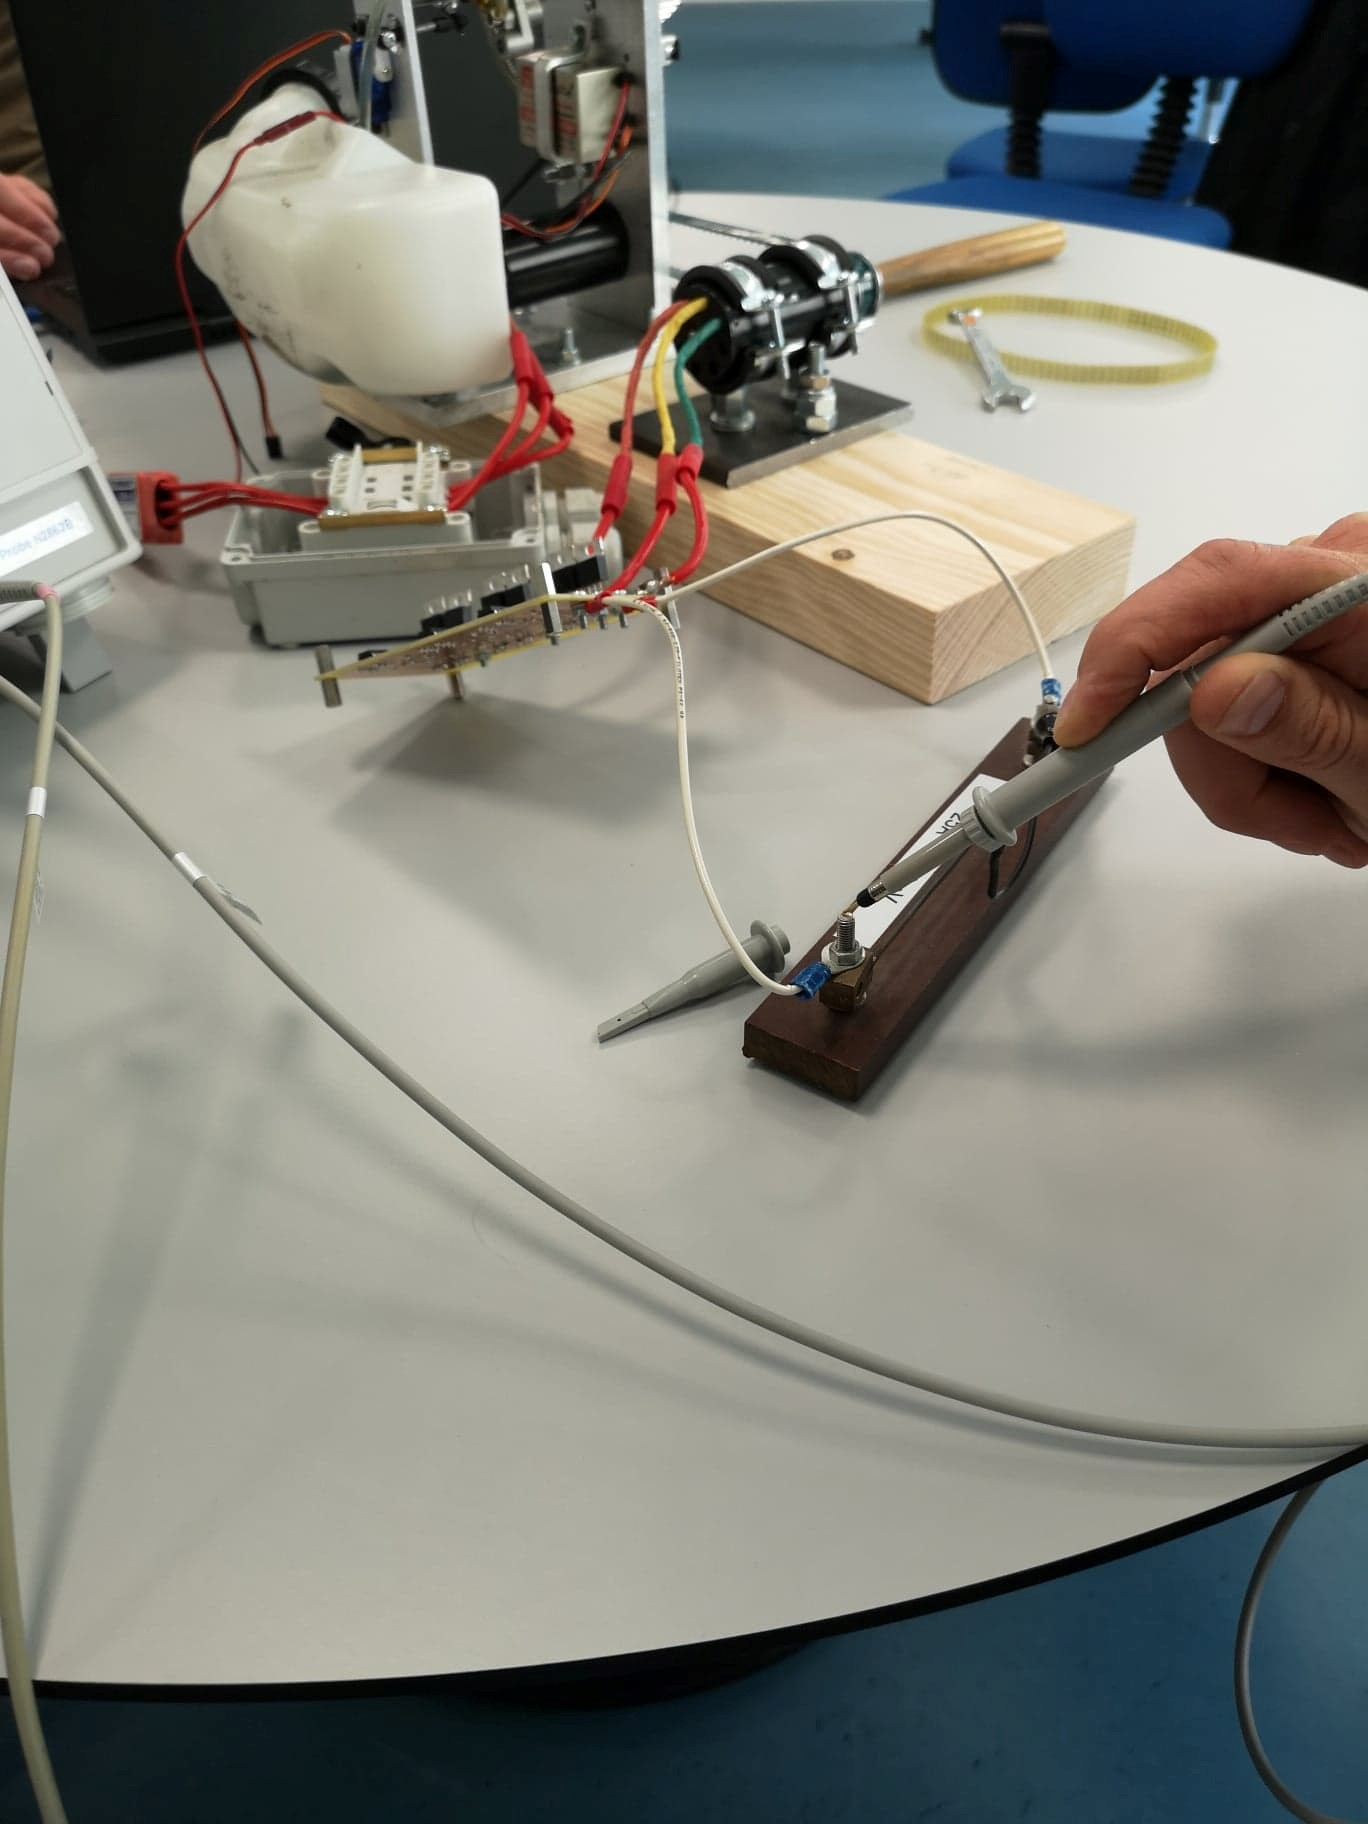
\includegraphics[width=0.6\textwidth]{tbil4.jpg}
  \caption{Foto af testopstilling med load modstand på ca. 12 m$\Omega$.}
  \label{fig:tbil4}
\end{figure}

Effektmodstanden er designet således, at der løber 25 A gennem den, hvis der er et spændingsfald på 300 mV over modstanden.  

Teststanden fra timebox 7 blev igen benyttet til at genere inputtet til ensretteren.

\begin{enumerate}
\item måling: Generatoren blev drevet således, der løb ca. 25 A gennem load modstanden.
\end{enumerate}
Efter få sekunder kunne vi konstatere, at de 6 MOSFETS på printet blev meget varme, hvorfor testen blev stoppet. 

De 6 MOSFETS på printet er af typen:
\begin{itemize}
\item Fairchild, FDP61N20, N-channel MOSFET\footnote{http://213.114.131.21/_pdf/FD/FDP61N20.pdf}
\item Drain-current: 61 A
\item Drain-source spænding: 200 V
\item RDS(ON) = 0.041 $\Omega$
\item VGS = 10 V
\item Thermal Resistance, J-A, $R_{\theta iA} = 62.5^\circ C/W$
\end{itemize}

Ud fra datasheet’et kan det ses, at den interne modstand i disse MOSFETS er på 41 m$\Omega$. Det er denne modstand, der forårsager spændingstabet fra faserne til outputtet. 

Hvis det antages, at der i værste fald er et spændingsfald på de tidligere beregnede 0.3497 V fra source til drain på hver af de 6 MOSFETS, vil dette resultere i et effekttab på 

\begin{equation}
  \label{eq:1}
  P = \frac{0.3497^2V}{0.041 \Omega}=2.87W
\end{equation}

Og dette vil aflede en stigning i temperaturen i de 6 MOSFETS på:
\begin{equation}
  \label{eq:2}
  T = P \cdot R_{\theta jA}=2.87 W\cdot 62.5 \frac{^\circ C}{W} = 179.2 ^\circ C
\end{equation}

Ud fra datasheet’et til FDP61N20 ses det, at disse MOSFETS maksimalt kan håndtere 150 $^\circ C$.

\subsection{Konklusion}
\label{sec:konklusion}

Ud fra funktionalitettesten af den aktive ensretter, hvor inputspænding vs. outputspænding plottes og spændingsfaldet beregnes i Matlab, kan det konkluderes, at kredsløbet lever op til kravet om ikke at have et spændingsfald på udgangen på mere end 0.7 volt i forhold til indgangen.  Det kan derfor konstateres, at den er væsentlig mere effektiv end en ensretter bestående af en diodebro.   

Spændingstabet ved anden måling af funktionalitetstesten er dog relativ høj i forhold den første måling (0.3497 V vs. 0.0967 V), hvilket forekommer besynderligt. Ideelt set burde spændingstabet være det samme ved samtlige inputspændinger, så forskellen kan muligvis forklares ud fra en uregelmæssighed på én eller flere af de tre faser fra generatoren, der producerer inputsignalet til kredsløbet. 

Derudover kan der konkluderes, at valget af MOSFET til realiseringen af ensretter-printet skal ændres. De nuværende MOSFETS kan ikke leve op til varmeafledningen, hvorfor der skal vælges andre MOSFETs med en lavere intern modstand og evt. påmonteres køleplader til disse. 
Dette vil blive testet og redegjort for i næste timebox. Den endelige test af max belastning forventes ligeledes gennemført i timebox 10. 
    
\clearpage

\section{Tuning af PID-koefficienter (Simon)}
\label{sec:tuning-af-pid}

I sidste timebox fandtes overføringsfunktionen
\begin{equation}
  \label{eq:1}
G(s) = \frac{8900}{0,04s+1}  
\end{equation}
I Simulink oprettes følgende:

\begin{figure}[h]
  \centering
  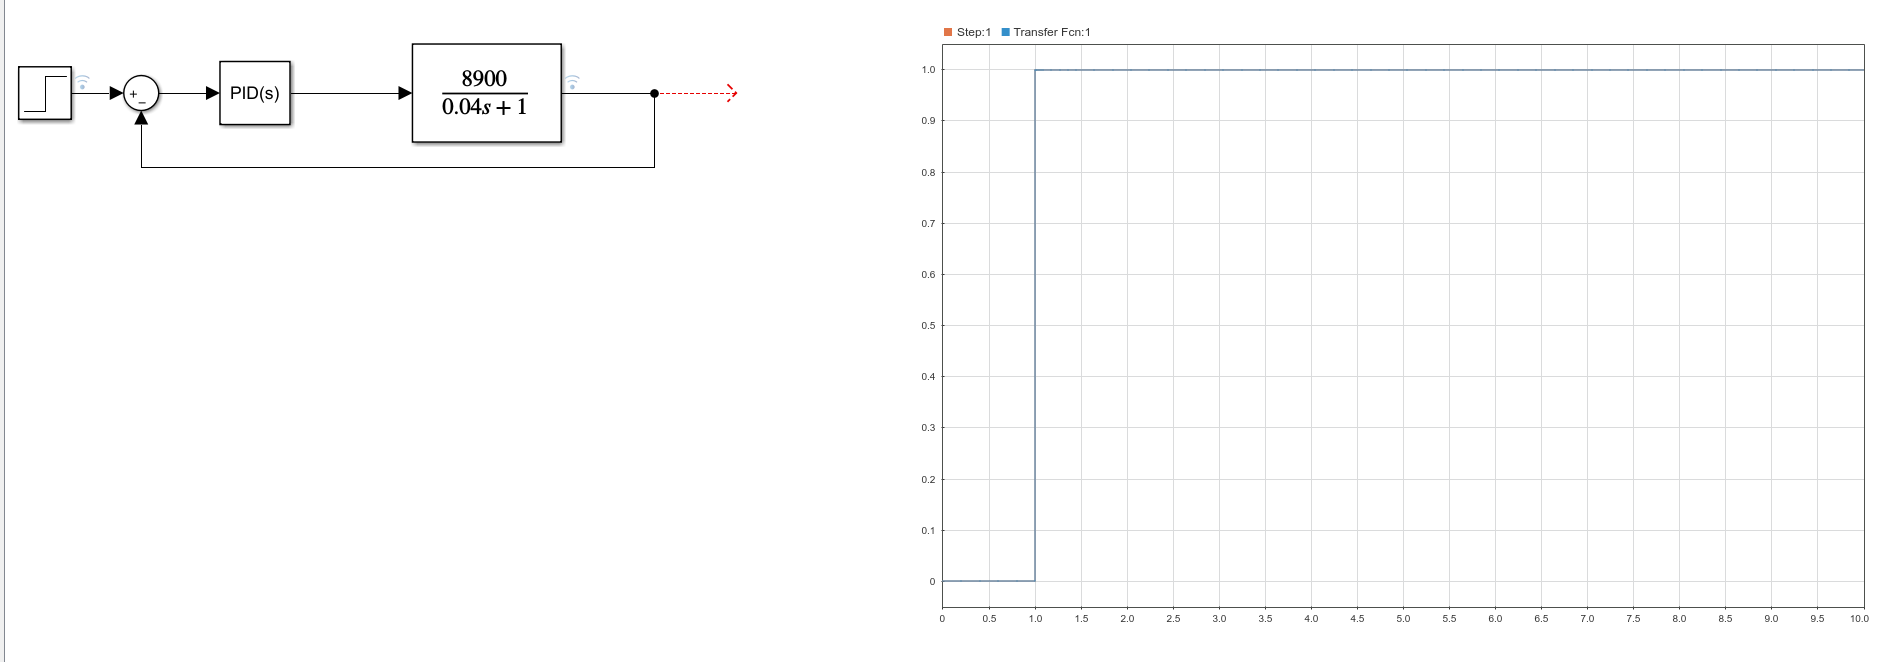
\includegraphics[width=0.6\textwidth]{sbil1.png}
  \caption{Simulink - diagram}
  \label{fig:sbil1}
\end{figure}

Herefter laves autotuning i PID-modulet. Der findes koefficienter svarende til $P=0,0010$, $I=0,0514$, $D=-1,4946$ og følgende respons:

\begin{figure}[h]
  \centering
  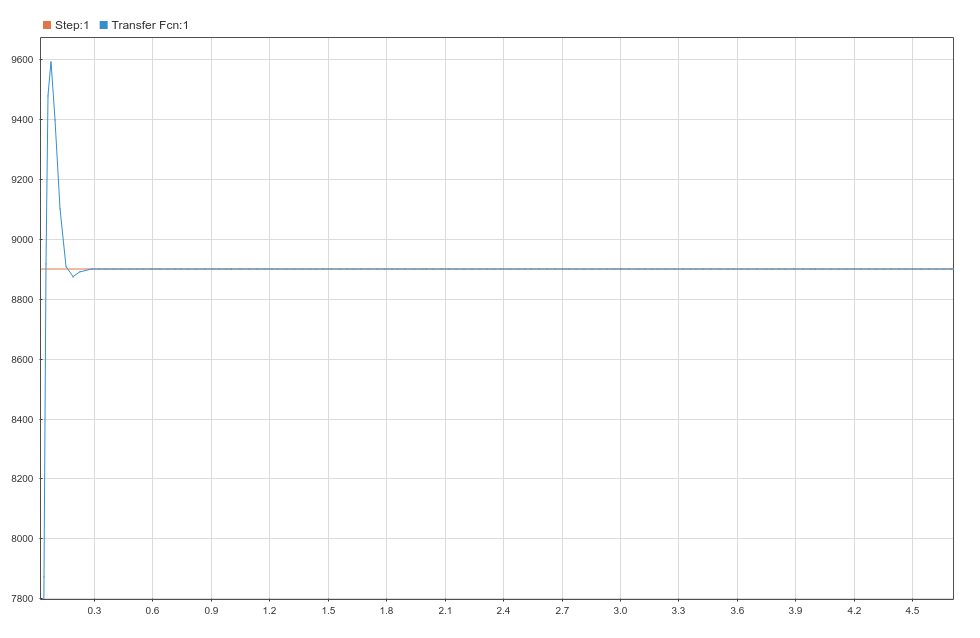
\includegraphics[width=0.6\textwidth]{sbil2.png}
  \caption{Simulink - diagram 2}
  \label{fig:sbil1}
\end{figure}

I næste timebox implementeres og justeres PID-reguleringen.
\clearpage
\section{Deployment (Alle)}
\label{sec:deployment}

I denne timebox deployes en opnået spændingsregulering fra 22 V til 5,3 V. Herudover deployes udkast til kode der skal aflæse omdrejningstal fra forbrændingsmotoren og desuden deployes de tunede PID-koefficienter.

Hermed godkender kunderne, Morten Oppbrud Jakobsen og Jan Møller Nielsen, ovenstående i timebox 9.

Mandag den 13/5-2019

\begin{minipage}{.5\textwidth}
  \begin{center}
    \vspace{1.4cm}
    \rule{0.8\textwidth}{0.1pt}\\
    \small{Morten Opprud Jakobsen\\%\vspace{0.1cm}\textit{Projektansvarlig læge}
    }
  \end{center}
\end{minipage}%
\begin{minipage}{0.5\textwidth}
  \begin{center}
    \vspace{1.4cm}
    \rule{0.8\textwidth}{0.1pt}\\
    \small{Jan Møller Nielsen\\%\vspace{0.1cm}\textit{Forskningsansvarlig overlæge}
    }
  \end{center}
\end{minipage}

% \printbibliography
\end{document}